\section{The angular distribution for higher \kpi states}
\label{sec:kpistates}

The angular distribution of \BdToKstll depends strongly on the spin of the \kpi state and measurements
of angular observables require the P-wave \kpi state, oh which the \Kstarz(892) is the dominant mode.
There are several \Kstarz states which decay strongly to \kpi with masses similar to the \Kstarz(892) which could
possibly affect the narrow width assumption assumed by many theoretical papers and any angular analysis of \BdToKstll.
The \kpi line shape in an angular analysis of \BdToKstll has previously been considered in Refs~\cite{Grinstein:2005ud,Lu:2011jm,Li:2010ra}.
The different resonant \Kstarz states known to decay strongly to \kpi with a high branching fraction are detailed in Table~\ref{kpistates}.
\begin{table}[htbp]
\centering
\caption{ Data for resonant \Kstarz states which decay strongly to \kpi with masses around 1\gev~\cite{PDG2012}. 
The evidence for a $\kappa(800)$ is inconclusive. ~\label{kpistates} }
\begin{tabular}{|c|c|c|c|c|}
\hline
State & Mass (\mev) & $\Gamma$ (\mev) & $\Gamma_{\Kstarz\to\kpi}$ (\mev) & Phase \\
\hline
\Kstarzo(892) &$ 895.94\pm0.22 $&$ 48.7\pm0.8 $&$ 100\% $&$ 0 $\\
\Kstarzz(1430) &$ 1430\pm50     $&$ 270\pm80   $&$ 100\% $&$ 0 $\\
\Kstarzt(1430) &$ 1432.4\pm1.3  $&$ 109\pm5    $&$ 50\%  $&$ 0 $\\
\Kstarzo(1680) &$ 1717\pm27     $&$ 322\pm100  $&$ 40\%  $&$ 0 $\\
\hline
$\kappa(800) $&$ 800  $&$ 600   $&$ 100\% $&$ 0 $\\
\hline
\end{tabular}
\end{table}
There exists partial evidence for both a low mass spin-0 $\kappa(800)$ 
or a generic non resonant \kpi contribution at masses below 1\gev.
There are four states along with a possible low mass spin-0 $\kappa(800)$. 
The existence of this state is uncertain and it has been considered to be non-resonant \kpi contribution~\cite{PDG2012}.

\subsection{propagator functions}

Each of these functions can be described by a relativistic Breit-Wigner  distribution [ REFERENCE ].
\begin{itemize}
    \item Explain BW
\end{itemize}
Several parametrisation have been suggested to model the \kpi line shape correctly, of which the LASS parametrisation~\cite{Aston:179353} is one. 
\begin{itemize}
\item pros, cons 
\end{itemize}
Another is to use an isobar model, combining each of the different resonances~\cite{PhysRevLett.89.121801}.

\begin{itemize}
\item Explain propagators?
\item LASS
\item Relativistic Breit Wigner
\item \dots
\end{itemize}

\subsection{\psq spectrum}

In the \psq region between threshold and up to 2\gevgevcccc there are contributions from the S-, P- and D-waves.
Contributions from \Kstarz states with resonant masses above 1600\mev can be ignored and the \Kstarzo(1410) does 
not decay dominantly to \kpi.
The \psq spectrum of the angular distribution for this combination of the S, P and D-wave is given in
Fig~\ref{fig:psq:spdwave}.
\begin{figure}[tbp]
\centering
\subfigure{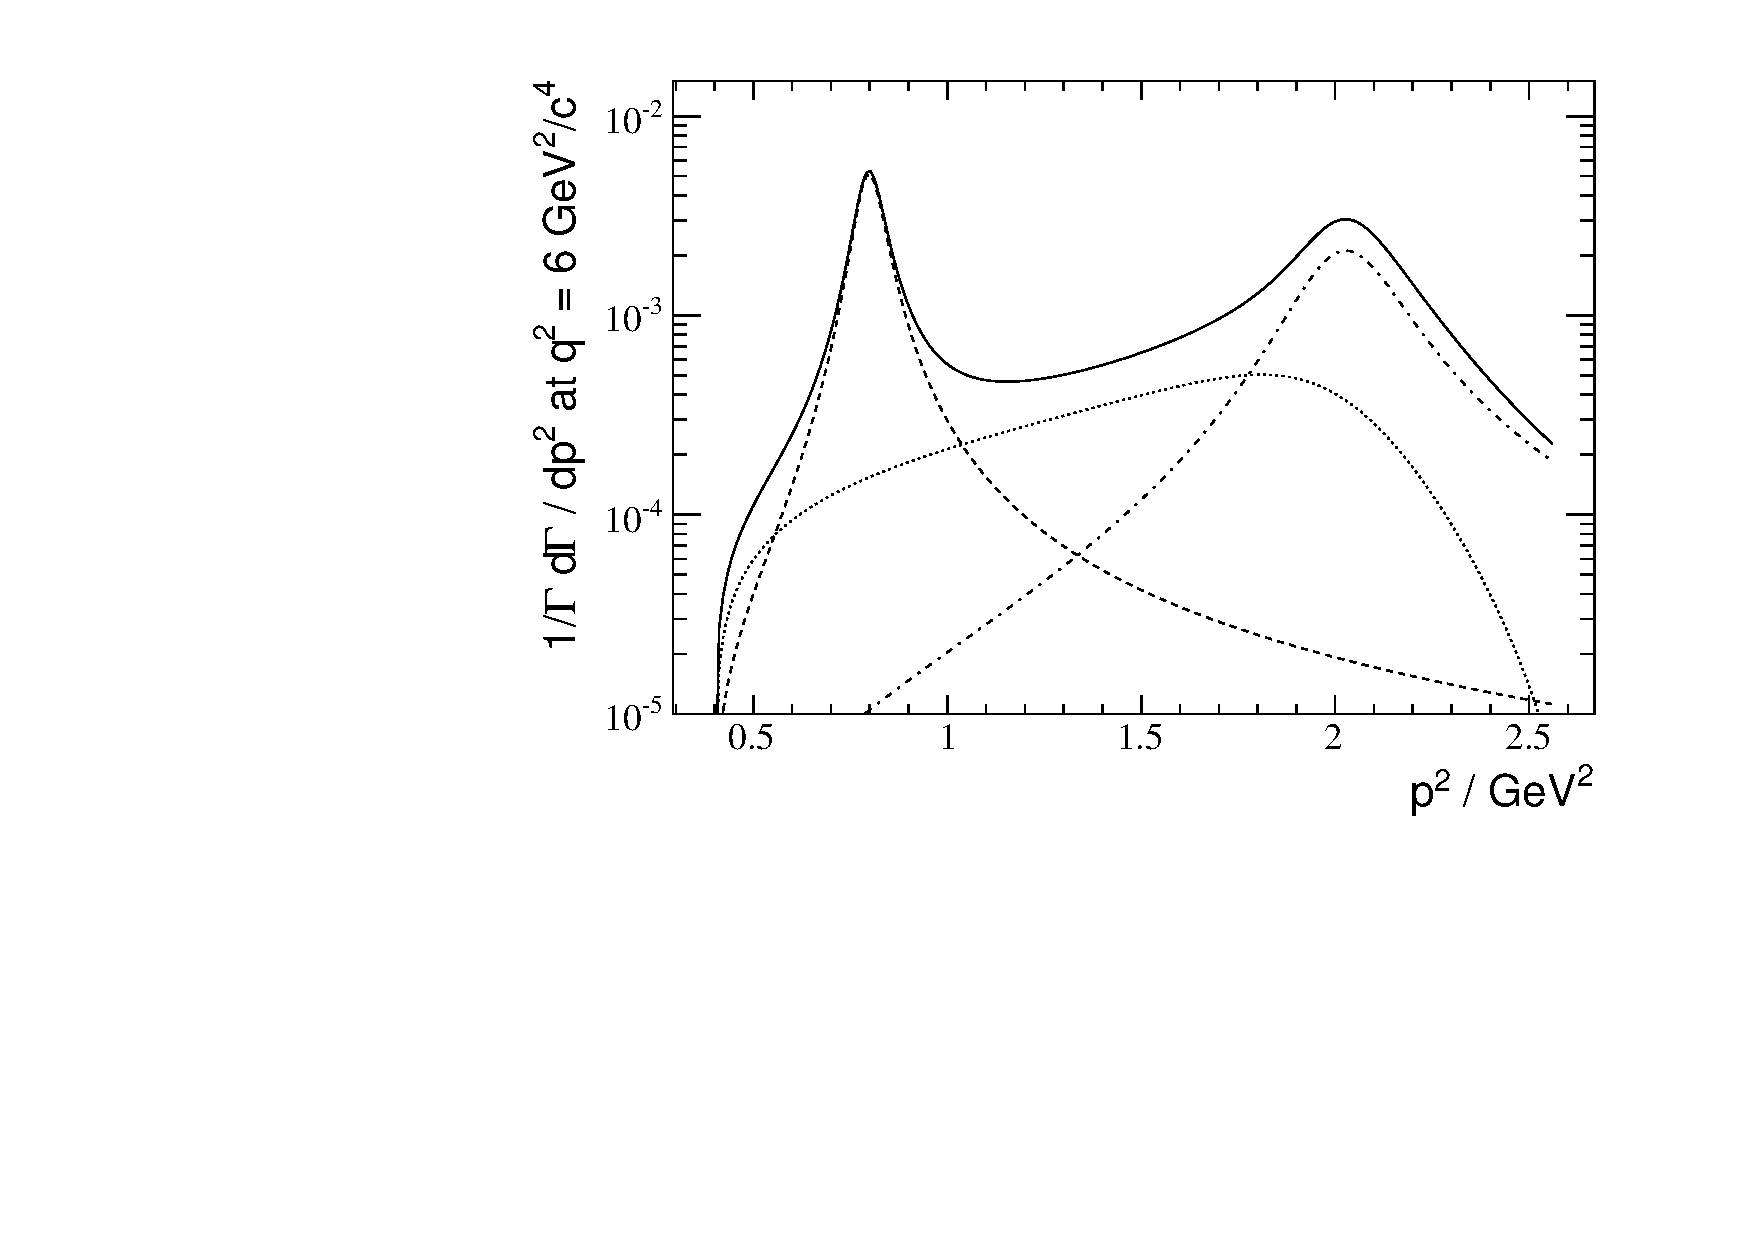
\includegraphics[width=0.48\columnwidth]{chapter4/figs/calc_psq_branch_frac_logy.pdf}}
\caption{ The total branching fraction for \BdToKpill in the region from threshold to 2.5\gevgevcccc where there are dominant contributions
from the S-,P and D-waves. Equal matrix elements are used for each state and the complete distribution is normalised to unity.
  ~\label{fig:psq:spdpwave} }
\end{figure}
It is possible to see the negligible contribution from the D-wave in the mass region close to the peak of the P-wave. 
The effect of S-wave interference in the P-wave region is explored in Chapter~\ref{chap:swave}.

Each of the multiple \Kstarz states will affect the angular distribution in \ctk.
The two dimensional angular distribution of the \psq and \ctk for two combinations of \Kstarz states is shown in Fig~\ref{fig:ctk:spdwave}.
\begin{figure}[tbp]
\centering
\subfigure{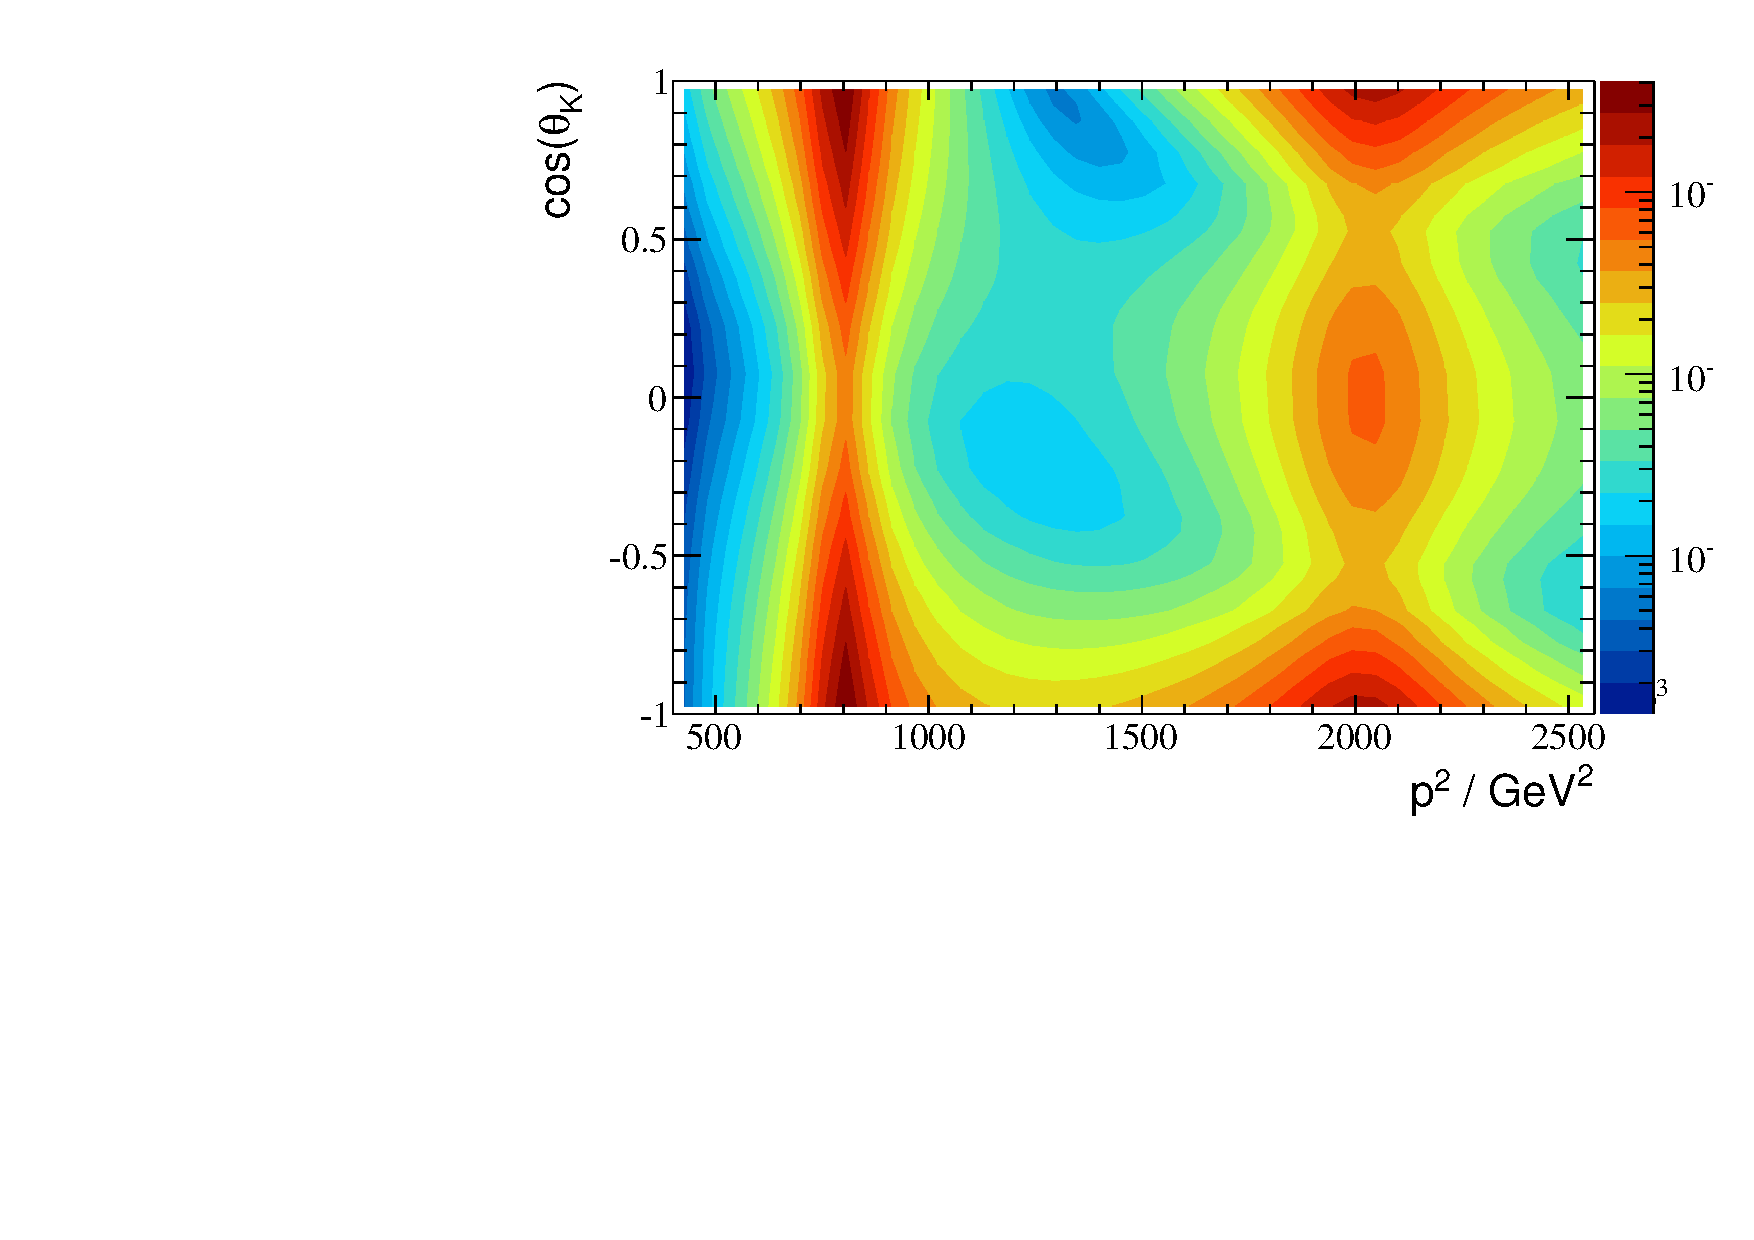
\includegraphics[width=0.48\columnwidth]{chapter4/figs/calc_ctk_psq_branch_frac_logy_pd.pdf}}
\subfigure{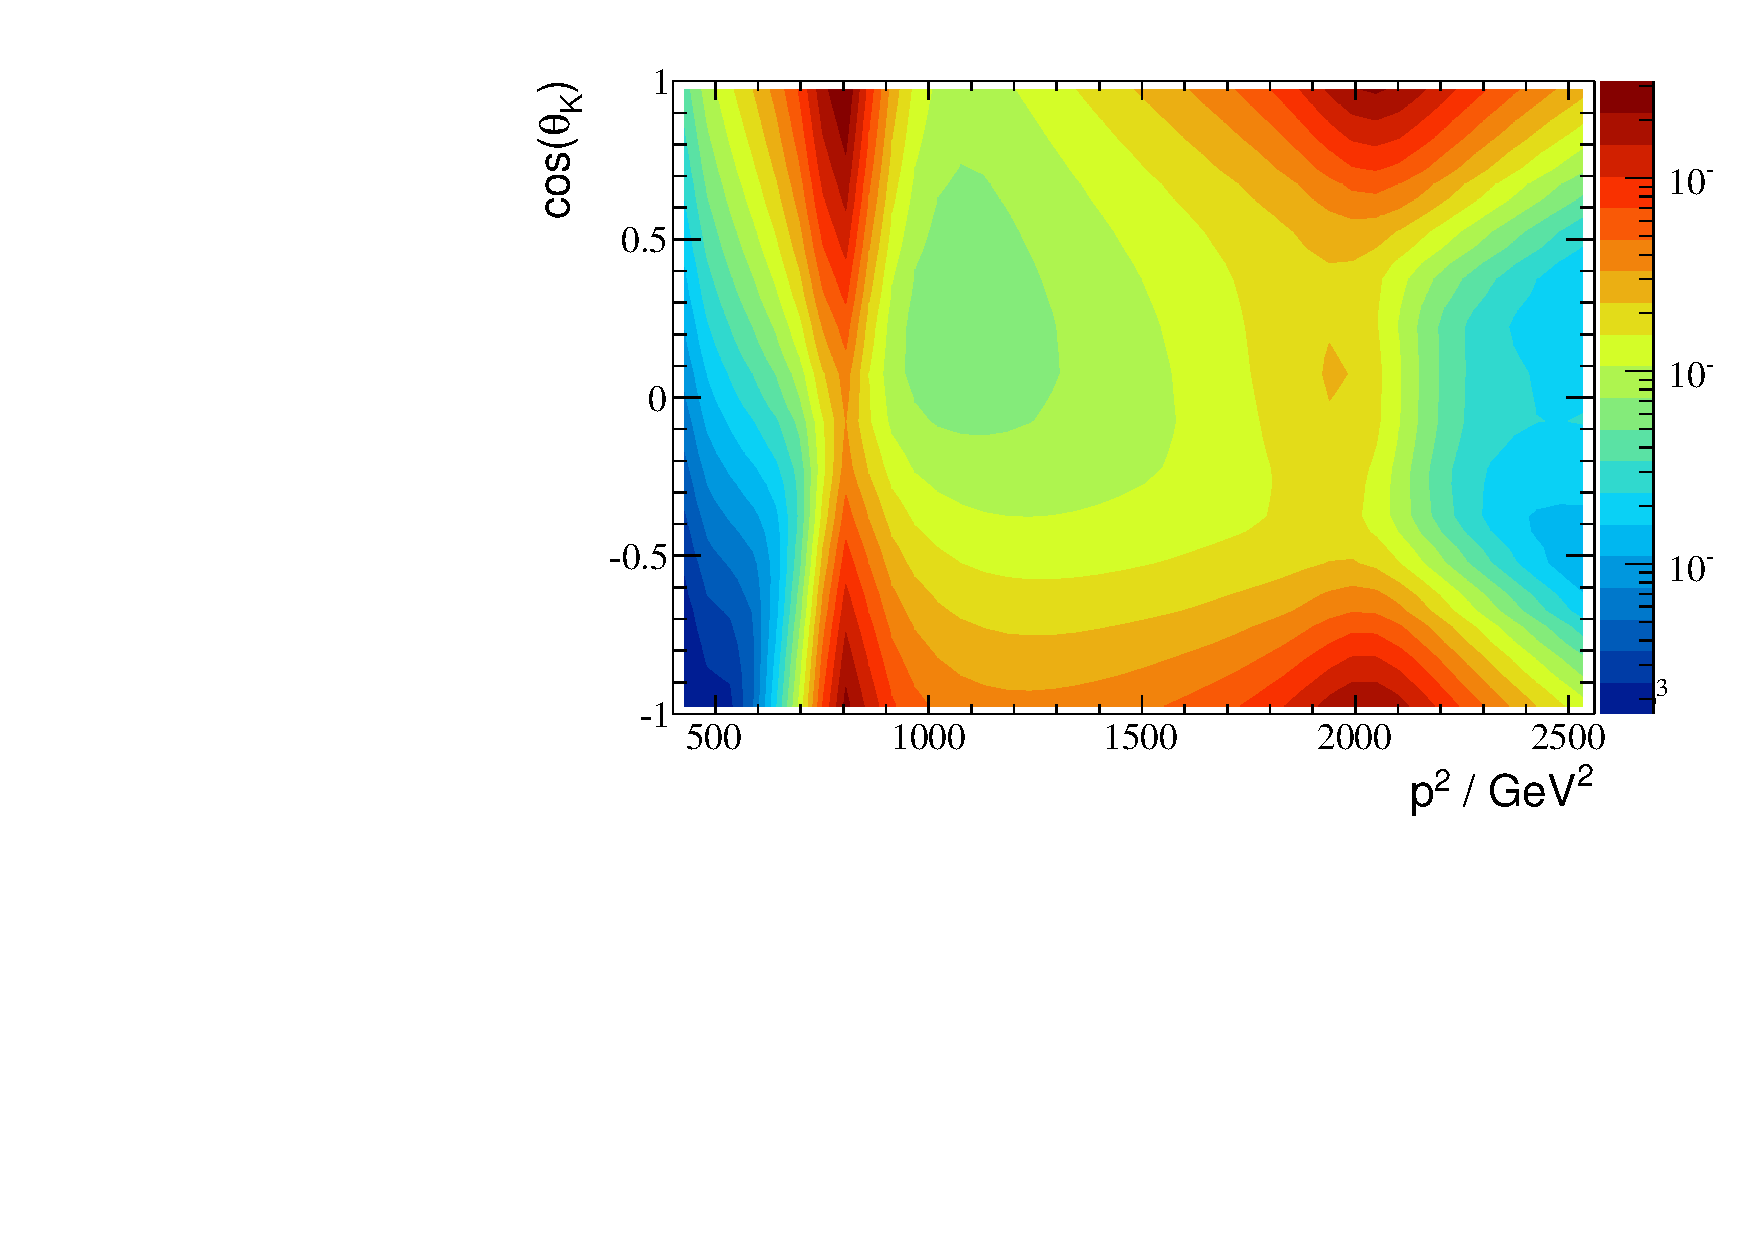
\includegraphics[width=0.48\columnwidth]{chapter4/figs/calc_ctk_psq_branch_frac_logy.pdf}}
\caption{ ~\label{fig:ctk:spdwave} }
\end{figure}
It is possible to see that for a combination of the P and D-waves, there is quite a clear distinction between
the different harmonics at each resonant mass.
For the combination of S,P and D-waves there is an consistent asymmetry across all of \psq, affecting the 
P-wave slightly but dramatically washing out the D-wave.

\subsection{Angular distribution of the S,P and D-wave}


see Appendix~\ref{fullangulardistribution}.



\subsection{Angular observables for the D-wave }

The angular observables for the \kpi D-wave follow the same structure 
as the angular observables for the P-wave. 
For example, it is possible to define a forward-backward dimuon asymmetry 
and the longitudinal polarisation of the \Kstarz as
\begin{equation}
\begin{split}
\label{eq:theodobs}
\AFBD(\qsq) &= \frac{3}{2} \frac{  \Re(A_{2L||}A_{2L\bot}^{*}) - 
\Re(A_{2R||}A_{2R\bot}^{*})}{|A_{20}|^2 + |A_{2||}|^2 + |A_{2\bot}|^2 } \\
\FLD(\qsq) &= \frac{  |A_{20}|^2 } {|A_{20}|^2 + |A_{2||}|^2 + |A_{2\bot}|^2} ,
\end{split}
\end{equation}

The total angular distribution is normalised to all the \kpi amplitudes,
\begin{align}
\Gamma = \sum_{J,(0,||,\bot)} |A_{J,(0,||,\bot)}|^2
\end{align}
so each of the P and D-wave observables are accompanied by the relative branching fraction, given by \FPi or \FDi respectively.
The proportion of each \kpi state compared to the total branching fraction is given by
\begin{subequations}\begin{align}
\FSi(\psq,\qsq) &= \left( \frac{|A_{00}|^2 }{\sum_{J,(0,||,\bot)} |A_{J,(0,||,\bot)}|^2} \right) \\
\FPi(\psq,\qsq) &= \left( \frac{|A_{10}|^2 + |A_{1||}|^2 + |A_{1\bot}|^2 }{\sum_{J,(0,||,\bot)} |A_{J,(0,||,\bot)}|^2} \right) \\
\FDi(\psq,\qsq) &= \left( \frac{|A_{20}|^2 + |A_{2||}|^2 + |A_{2\bot}|^2 }{\sum_{J,(0,||,\bot)} |A_{J,(0,||,\bot)}|^2} \right) 
\end{align}\end{subequations}
The D-wave interferes with both the S-wave and the P-wave states.
The SD-wave interference can be expressed in a similar fashion to the 
SP-wave interference, through a single asymmetry
\begin{align}
\ASDi(\psq,\qsq)  &= \frac{\sqrt{3}}{2} \left( \frac{ |A_{0L0}||A_{1L0}|\cos\delta_L
+ (L\to R)}{|A_{10}|^2 + |A_{1||}|^2 + |A_{1\bot}|^2 + |A_{00}|^2}\right)
\end{align}
The P-D interference is more complicated and occurs between both longitudinal and transverse amplitudes.
However, the size of this interference is small due to the separation between the two states, shown in Fig~\ref{fig:psq:spdpwave}, 
and the angular functions that contain \FPi and \FDi simultaneously can be ignored.

The angular distributions with these angular observables are given in Appendix~\ref{fullangulardistribution:obs}.

